
\begin{frame}{What is artificial intelligence?}
    \begin{tikzpicture}
        \node[] at (-7, -3.25) {};
        \node[] at (7, 3.25) {};

        \only<1>{
            \node[anchor=west, inner sep=0pt, draw=black, label=below:\tiny{ChatGPT}] at (-7, 0) {
                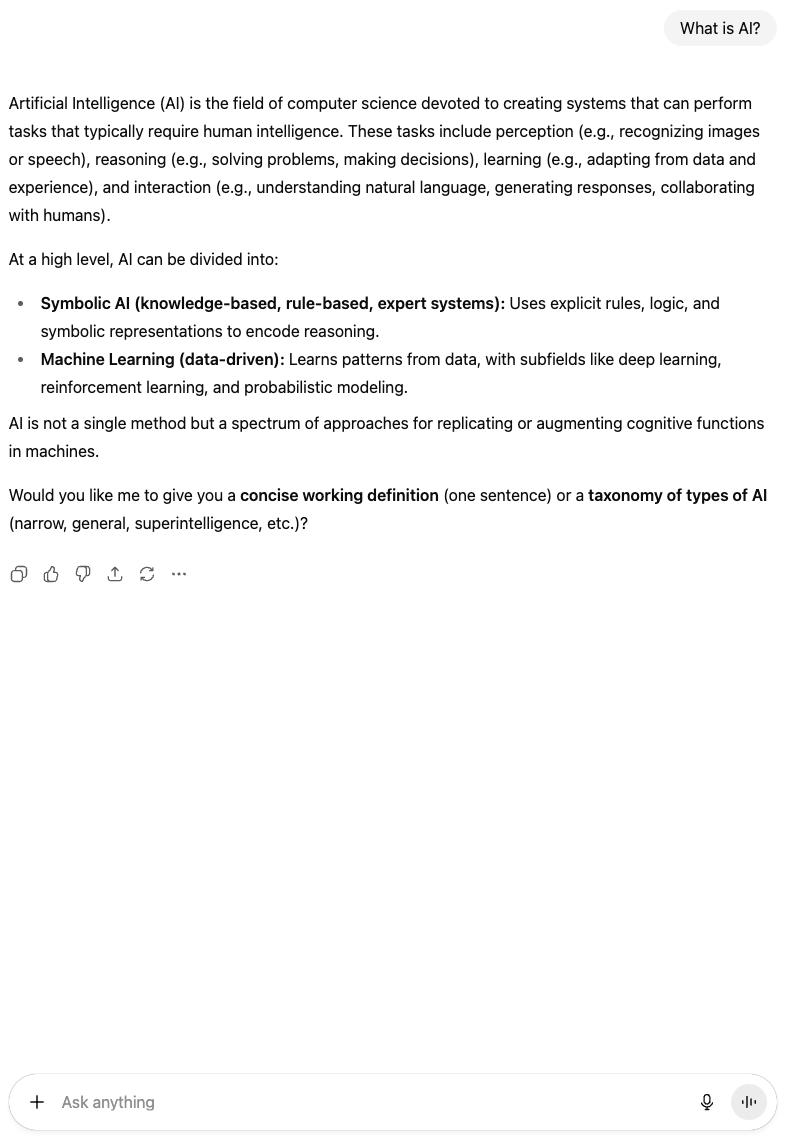
\includegraphics[width=4.1cm]{data/chatgpt.png}
            };
            \node[inner sep=0pt, draw=black, label=below:\tiny{Spot}] at (-0.5, 1.5) {
                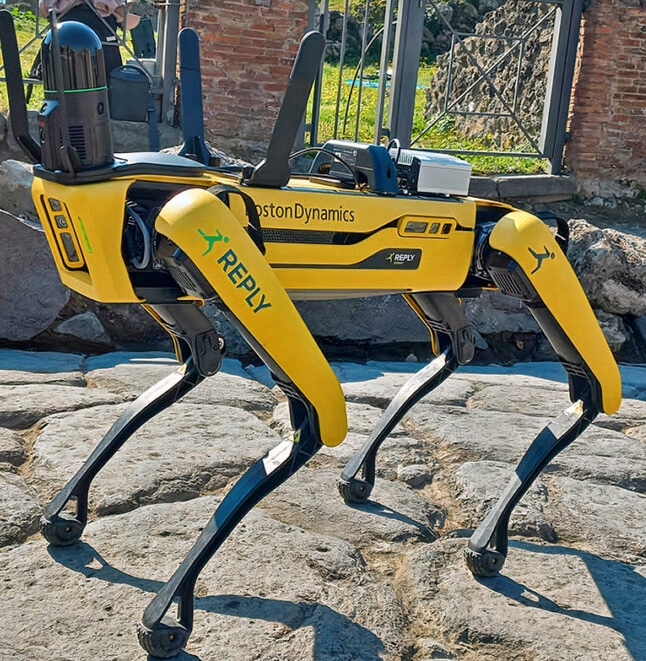
\includegraphics[width=2.5cm]{data/spot.jpg}
            };
            \node[inner sep=0pt, draw=black, label=below:\tiny{Sophia}] at (2.7, 1.9) {
                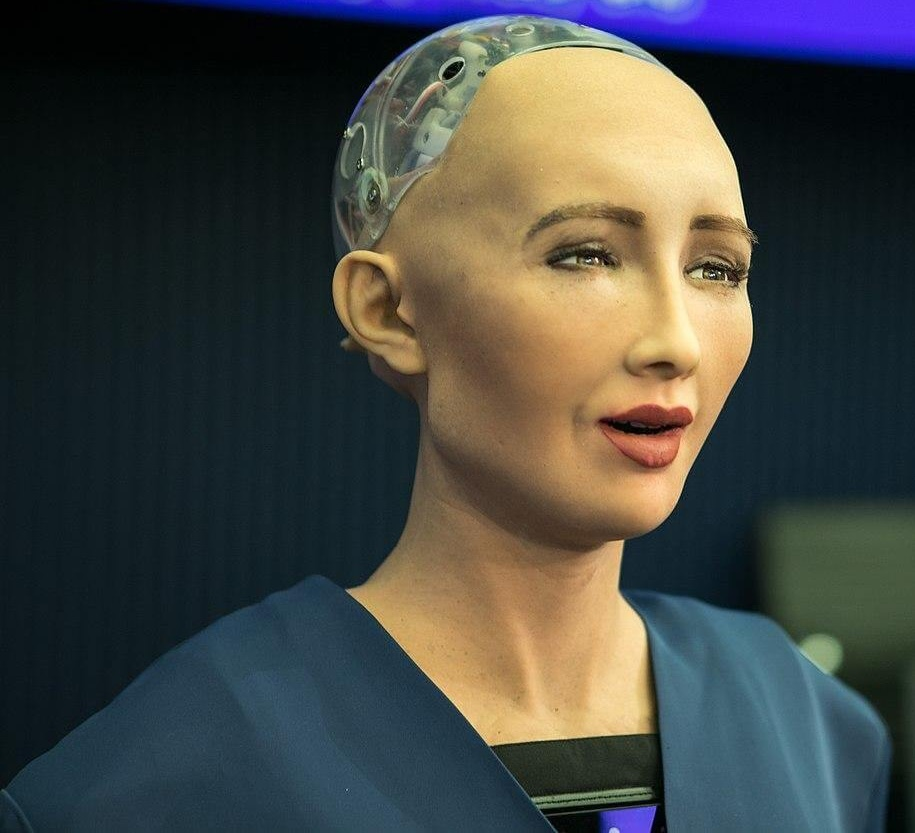
\includegraphics[width=2.5cm]{data/sophia.jpg}
            };
            \node[inner sep=0pt, draw=black, label=below:\tiny{AlphaFold}] at (1, -1.8) {
                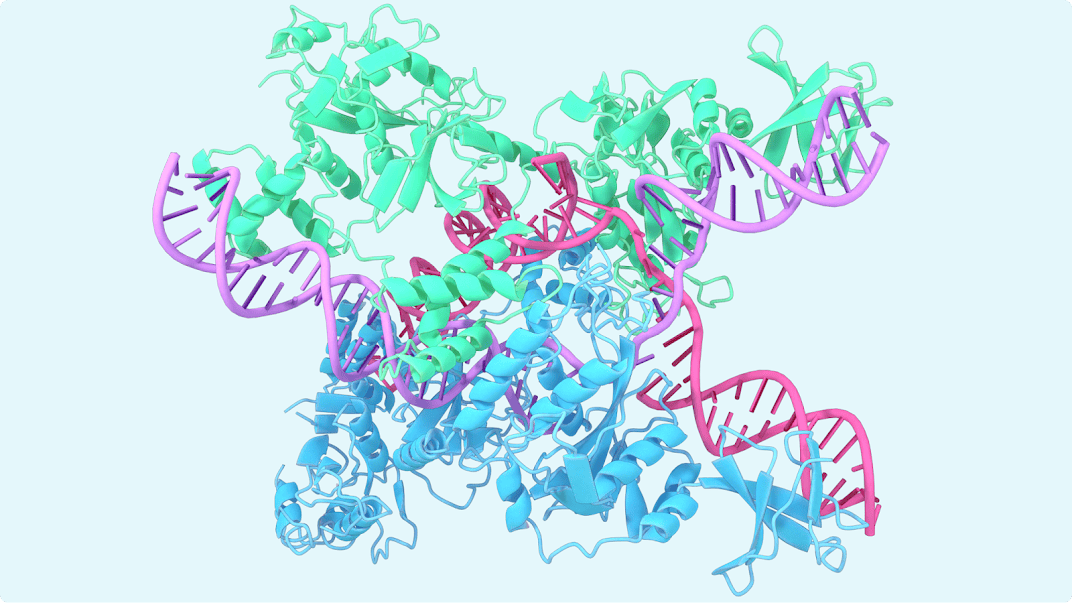
\includegraphics[width=3cm]{data/alphafold.png}
            };
            \node[inner sep=0pt, draw=black, label=below:\tiny{AlphaZero}] at (4.5, -1.1) {
                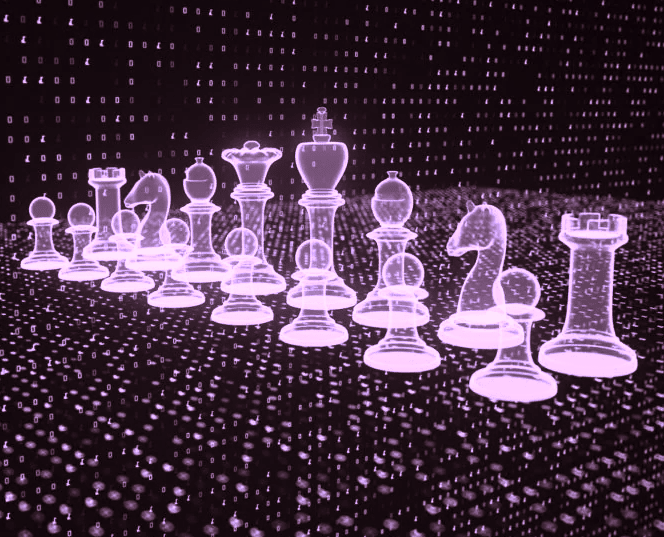
\includegraphics[width=2.7cm]{data/chess.png}
            };
        }

        \only<2>{
            \node[circle, fill=uioblue!80, minimum size=6cm, anchor=north] (ai) at (-4, 3.25) {};
            \node[white, anchor=north, align=center, font=\small\bfseries\linespread{0.9}\selectfont] at ($ (ai.north) - (0, 0.1) $) {Artificial\\intelligence};
            \node[align=flush left, anchor=north west, text width=7.2cm, font=\small\linespread{0.95}\selectfont] (def1) at (-0.5, 3.25) {
                \textbf{Artificial intelligence}\\
                The field of study producing technology that solves tasks requiring some form of intelligence
            };
            \node[circle, fill=uioblue!50!uiored!80, anchor=south, minimum size=4.1cm] (ml) at ($ (ai.south) + (0, 0.05) $) {};
            \node[white, anchor=north, align=center, font=\small\bfseries\linespread{0.9}\selectfont] at ($ (ml.north) - (0, 0.1) $) {Machine\\learning};
            \node[align=center, font=\small\linespread{0.9}\selectfont, text=white] at ($ (ai.north) + (1.3, -1.5) $) {Rule-based\\systems};
            \node[align=flush left, anchor=north west, text width=7.2cm, font=\small\linespread{0.95}\selectfont] (def2) at (def1.south west) {
                \textbf{Machine learning}\\
                A set of techniques to solve problems by allowing machines to find patterns in training data
            };
            \node[circle, fill=uiored!80, anchor=south, minimum size=3cm] (dl) at ($ (ml.south) + (0, 0.06) $) {};
            \node[white, anchor=north, align=center, font=\small\bfseries\linespread{0.9}\selectfont] at ($ (dl.north) - (0, 0.1) $) {Deep\\learning};
            \node[align=flush left, anchor=north west, text width=7.2cm, font=\small\linespread{0.95}\selectfont] (def3) at (def2.south west) {
                \textbf{Deep learning}\\
                    Machine learning approaches that rely on artificial neural networks
                };

        }
    \end{tikzpicture}
\end{frame}

\newcommand{\brainsize}[1]{
    \begin{tikzpicture}
        \begin{axis}[
            width=8cm,
            height=3.8cm,
            xlabel=\footnotesize{Age},
            ylabel=\footnotesize{Brain size},
            xmajorticks=false,
            ymajorticks=false,
            axis lines=left,
            xmin=2,
            xmax=13,
            ymin=935,
            ymax=1600
        ]
            \addplot[
                only marks,
                uioblue,
                opacity=0.5
            ] table [
                col sep=comma,
                x=x,
                y=y
            ] {data/brainsize.csv};

            \ifnum#1=1
                \addplot[
                    samples=100,
                    domain=2:15,
                    very thick,
                    uioblue
                ] {
                    1064.062904437416+x*36.95459273
                };
            \fi
            \ifnum#1=2
                \addplot[
                    samples=100,
                    domain=2:15,
                    very thick,
                    uioblue
                ] {
                    400+1100*(1-e^(-x/3))
                };
            \fi
        \end{axis}
    \end{tikzpicture}
}

\begin{frame}{Why do we use artificial neural networks?}
    \begin{tikzpicture}
        \node[] at (-7, -3.25) {};
        \node[] at (7, 3.25) {};

        \visible<1-3>{
            \node[anchor=east] (input) at (-3, 1.25) {$\text{input}$};
            \node[anchor=west] (output) at (3, 1.25) {$\text{output}$};
        }
        \visible<2>{
            \node[] at (-0.25, -1.85) {
                \brainsize{0}
            };
        }
        \visible<3>{
            \node[] at (-0.25, -1.85) {
                \brainsize{2}
            };
        }
        \visible<4>{
            \node[anchor=east, inner sep=0pt, draw=black] (input) at (-3, 1.25) {
                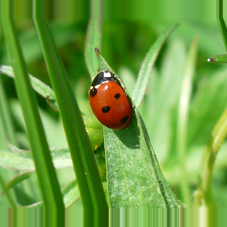
\includegraphics[width=2.5cm]{data/ladybug.png}
            };
            \node[anchor=west] (output) at (3, 1.25) {$\text{ladybug}$};
        }
        \visible<5>{
            \node[anchor=east, inner sep=0pt] (input1) at (-4, 2.75) {
                {\Huge{\emoji{spiral-notepad}}}
            };
            \node[anchor=east, inner sep=0pt, draw=black] (input2) at (-4, 1.25) {
                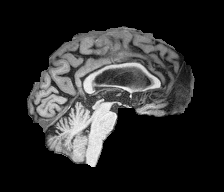
\includegraphics[width=1.5cm]{data/mri_sagittal.png}
            };
            \node[anchor=east, inner sep=0pt] (input3) at (-4, -0.25) {
                {\Huge{\emoji{microscope}}}
            };
            \node[anchor=west, align=left] (output) at (3, 1.25) {
                Clinical\\
                prediction
            };
        }

        \node[fill=gray!80, minimum width=4cm, minimum height=2.9cm, rounded corners=0.1cm, text=white, draw=black, font=\systemfont, anchor=south, text depth=2.4cm] (model) at (0, 0) {
            Artificial neural network
        };
        \only<1-4>{
            \draw[-stealth] (input.east) -- ($ (model.south west) + (0, 1.25) $);
        }
        \draw[-stealth] ($ (model.south east) + (0, 1.25) $) -- (output);
        \neuron{n00}{($ (model.south) + (0, 1.25) + (-2*\hsep, -2*\vsep) $)}
        \neuron{n01}{($ (n00) + (0, \vsep) $)}
        \neuron{n02}{($ (n00) + (0, 2*\vsep) $)}
        \neuron{n03}{($ (n00) + (0, 3*\vsep) $)}
        \neuron{n04}{($ (n00) + (0, 4*\vsep) $)}

        \neuron{n10}{($ (n00) + (\hsep, 0.5*\vsep) $)}
        \neuron{n11}{($ (n00) + (\hsep, 1.5*\vsep) $)}
        \neuron{n12}{($ (n00) + (\hsep, 2.5*\vsep) $)}
        \neuron{n13}{($ (n00) + (\hsep, 3.5*\vsep) $)}

        \neuron{n20}{($ (n00) + (2*\hsep, \vsep) $)}
        \neuron{n21}{($ (n00) + (2*\hsep, 2*\vsep) $)}
        \neuron{n22}{($ (n00) + (2*\hsep, 3*\vsep) $)}

        \neuron{n30}{($ (n00) + (3*\hsep, 1.5*\vsep) $)}
        \neuron{n31}{($ (n00) + (3*\hsep, 2.5*\vsep) $)}

        \neuron{n40}{($ (n00) + (4*\hsep, 2*\vsep) $)}

        \foreach \j in {0,...,4} {
            \draw[black, opacity=\edgeopacity] ($ (model.west) - (0, 0.2175) $) -- (n0\j);
        }

        \foreach \j in {0,...,4} {
            \foreach \k in {0,...,3} {
                \draw[black, opacity=\edgeopacity] (n0\j) -- (n1\k);
            }
        }
        \foreach \j in {0,...,3} {
            \foreach \k in {0,...,2} {
                \draw[black, opacity=\edgeopacity] (n1\j) -- (n2\k);
            }
        }
        \foreach \j in {0,...,2} {
            \foreach \k in {0,...,1} {
                \draw[black, opacity=\edgeopacity] (n2\j) -- (n3\k);
            }
        }
        \draw[black, opacity=\edgeopacity] (n30) -- (n40);
        \draw[black, opacity=\edgeopacity] (n31) -- (n40);
        \draw[black, opacity=\edgeopacity] (n40) -- ($ (model.south east) + (0, 1.25) $);

        \only<1>{
            \node[circle, draw=black, fill=uiogreen, minimum size=0.5cm] (neuron) at ($ (model.south) - (0, 1.5) $) {};

            \node[anchor=east, font=\scriptsize] (x1) at ($ (neuron) - (0.75, -0.5) $) {$\text{input}_1$};
            \node[anchor=east, font=\scriptsize] (x2) at ($ (neuron) - (0.75, 0) $) {$\text{input}_2$};
            \node[anchor=east, font=\scriptsize] (x3) at ($ (neuron) - (0.75, 0.5) $) {$\text{input}_3$};

            \node[anchor=west, font=\scriptsize] (y) at ($ (neuron) + (0.75, 0) $) {$\text{output}$};

            \draw[-stealth] (x1) -- (neuron);
            \draw[-stealth] (x2) -- (neuron);
            \draw[-stealth] (x3) -- (neuron);
            \draw[-stealth] (neuron) -- (y);

            \node[font=\small] at ($ (neuron) + (0, 1) $) {
                Artificial neuron
            };
        }

        \only<5>{
            \draw[-stealth] (input1) -- ($ (model.south west) + (0, 1.25) $);
            \draw[-stealth] (input2) -- ($ (model.south west) + (0, 1.25) $);
            \draw[-stealth] (input3) -- ($ (model.south west) + (0, 1.25) $);
        }
    \end{tikzpicture}
\end{frame}